%%%% fs-run-time-graph  Graph and its partitioning

\label {fs-graph}

In our model the dataflow is represented by a directed graph. This graph does not contain information about physical deployment, so further we call it {\it logical} graph. Each other node of the logical graph contains single operation, also called job or procedure. Edges show the order of these operations. The data items are processed one-by-one in a "streaming" manner.

Notably, despite the fact that commonly dataflow graphs assumed to be acyclic (DAGs) 
~\cite{Zaharia:2016:ASU:3013530.2934664, Carbone:2017:SMA:3137765.3137777},
our model does not have this restriction. Moreover, as we show further in this section, there are cases when cycles are required, e.g. for MapReduce-based algorithms. 

\subsection{Physical deployment and partitioning}

Each computational unit in our distributed runtime is assigned by integer interval. Intervals are not intersected and cover the range of 32-bit signed integer. Moreover, each unit contains complete logical graph.

Physical graph extends logical one by assigning hash function to each input of each operation. This hash function is applied to the payload of data items and determines partitioning. More precisely, the value of hash function is computed before next operation and corresponding data item is sent to the unit which is responsible for the computed value. Therefore, load balancing explicitly depends on the hash functions of the operations. Optimal balancing requires the knowledge of payload distribution. Hence, the hash functions are assigned by business logic.

Figure~\ref{logical-graph-figure} shows the example workflow of logical graph. Possible partitioning of this logical graph on two nodes is shown on the figure~\ref{physical-graph-figure}.

\begin{figure}[htbp]
  \centering
  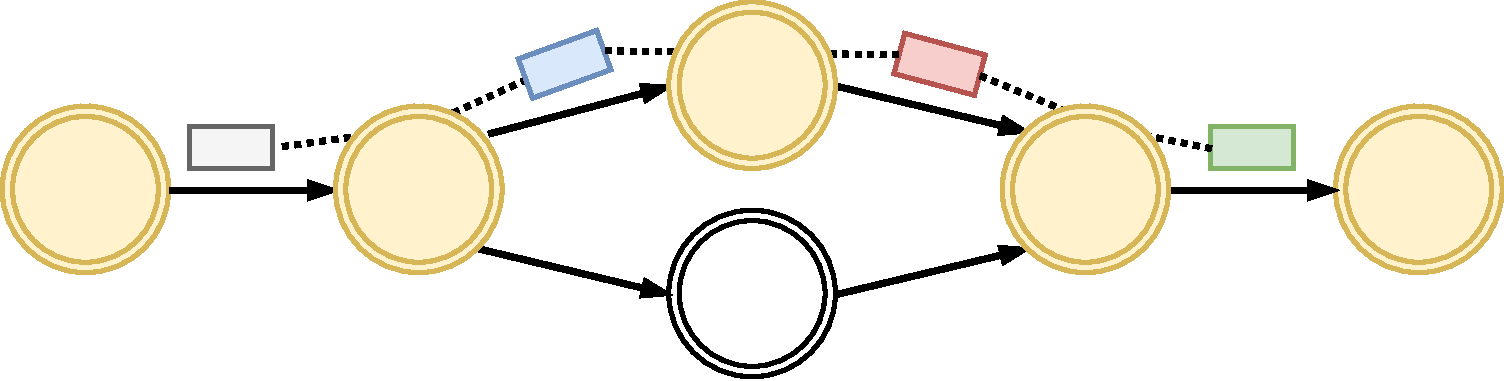
\includegraphics[width=0.48\textwidth]{pics/logical-graph}
  \caption{Logical graph workflow}
  \label {logical-graph-figure}
\end{figure}

\begin{figure}[htbp]
  \centering
  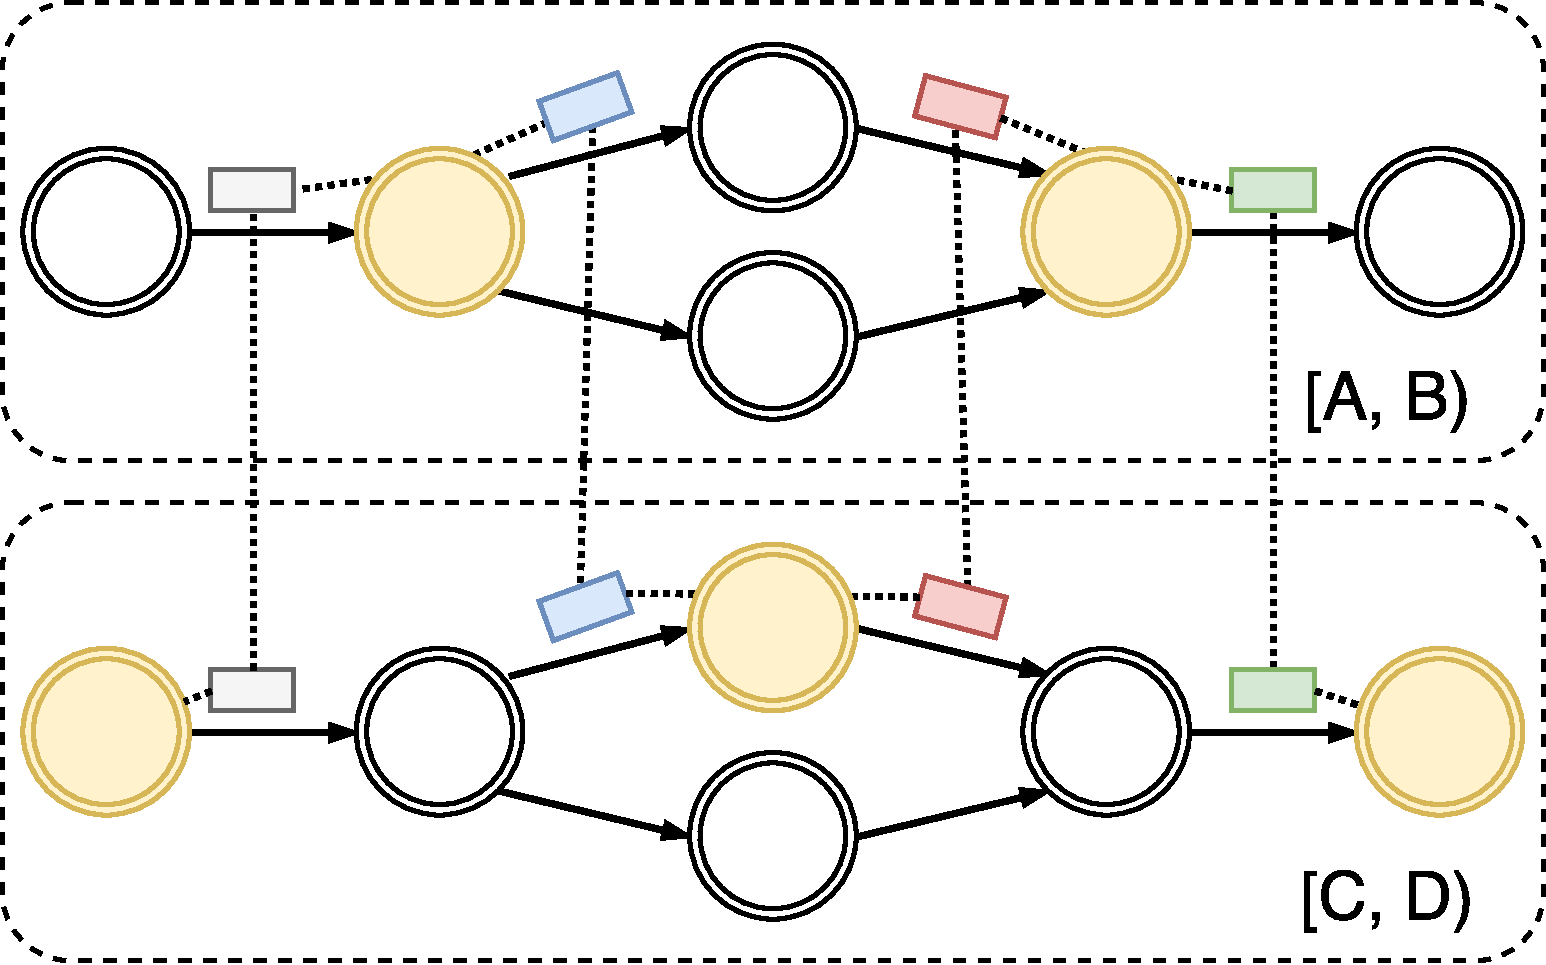
\includegraphics[width=0.48\textwidth]{pics/physical-graph}
  \caption{Possible partitioning of the logical graph}
  \label {physical-graph-figure}
\end{figure}
